\documentclass[10pt,border=1pt]{standalone}
\usepackage[T1]{fontenc}
\usepackage{mathpazo}
\usepackage{amsmath,amssymb}
\usepackage{xcolor}
\usepackage{pgfplots}
\pgfplotsset{compat=1.18}
\usetikzlibrary{shapes.geometric,positioning,arrows.meta,calc}
\definecolor{okorange}{HTML}{E69F00}
\definecolor{oksky}{HTML}{56B4E9}
\definecolor{okgreen}{HTML}{009E73}
\definecolor{okblue}{HTML}{0072B2}
\definecolor{okverm}{HTML}{D55E00}
\definecolor{okpurple}{HTML}{CC79A7}
\colorlet{accent}{okverm}
\pgfplotsset{
  safenest/.style={
    tick label style={font=\footnotesize},
    label style={font=\small},
    title style={font=\small, align=left},
    legend style={font=\footnotesize, draw=none, fill=none, cells={anchor=west}},
    grid style={black!12, line width=0.3pt},
    axis line style={black!70, line width=0.4pt},
    tick style={black!70, line width=0.4pt},
    axis lines*=left,
  },
}
\newlength{\figwidth}
\tikzset{every node/.append style={execute at begin node={\hyphenpenalty=10000\exhyphenpenalty=10000\relax}}}
\setlength{\figwidth}{18.47cm}
\begin{document}
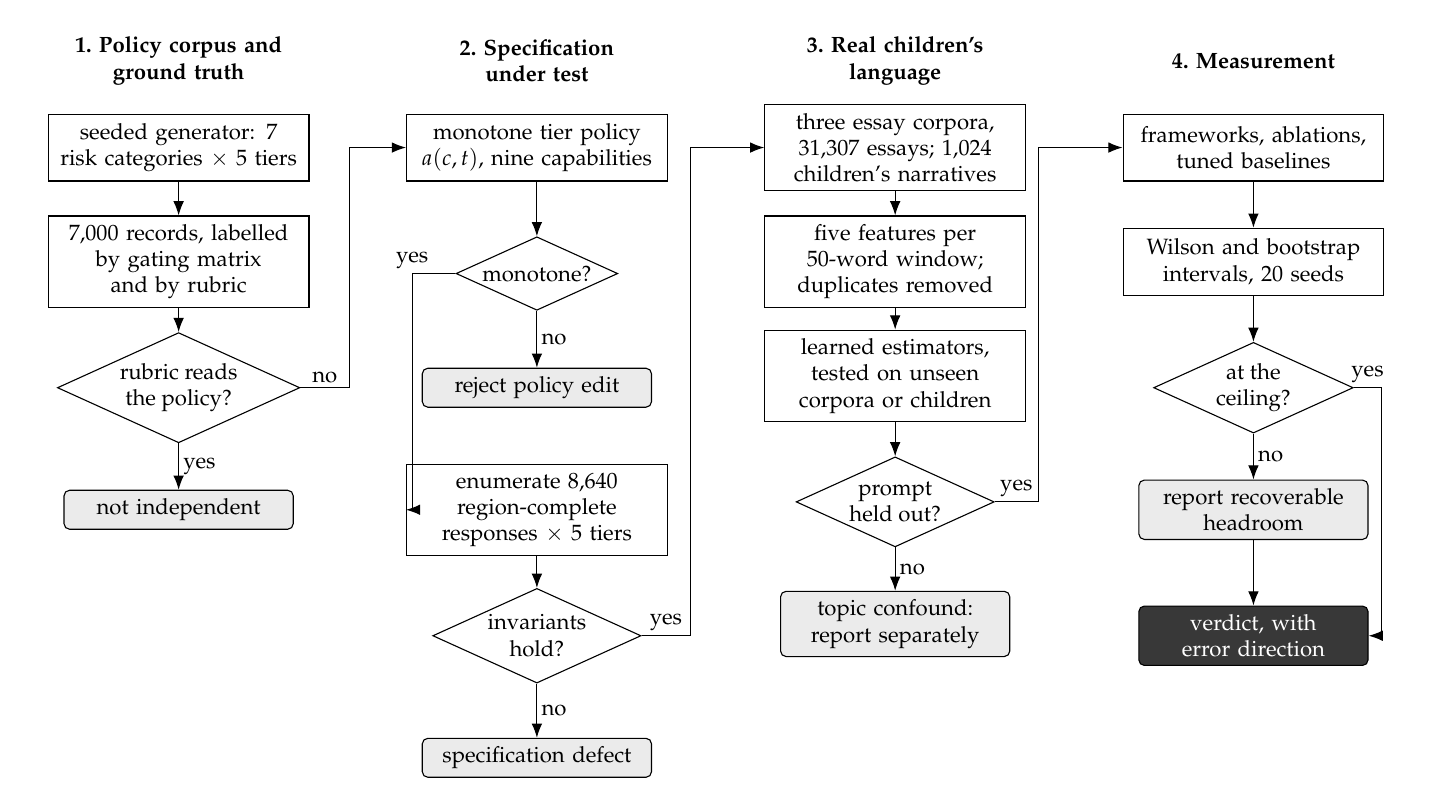
\begin{tikzpicture}[
  box/.style={draw, thin, rectangle, text width=31mm, align=center, inner sep=3pt,
              minimum height=8.5mm, font=\footnotesize},
  dec/.style={draw, thin, diamond, aspect=2.2, align=center, inner sep=1pt,
              font=\footnotesize},
  term/.style={draw, thin, rectangle, rounded corners=2pt, fill=black!8, align=center,
               inner sep=3pt, font=\footnotesize, text width=27mm},
  hd/.style={font=\footnotesize\bfseries, align=center, text width=36mm},
  ar/.style={-{Latex[length=1.8mm]}, thin},
  lb/.style={font=\footnotesize, inner sep=1.5pt},
]
\node[hd] at (0,0.1) {1.\ Policy corpus and\\ground truth};
\node[box] (a1) at (0,-1.0) {seeded generator: 7 risk categories $\times$ 5 tiers};
\node[box] (a2) at (0,-2.45) {7{,}000 records, labelled by gating matrix and by rubric};
\node[dec] (a3) at (0,-4.05) {rubric reads\\the policy?};
\node[term] (a4) at (0,-5.6) {not independent};
\draw[ar] (a1) -- (a2); \draw[ar] (a2) -- (a3);
\draw[ar] (a3) -- node[lb,right] {yes} (a4);

\node[hd] at (4.55,0.1) {2.\ Specification\\under test};
\node[box] (b1) at (4.55,-1.0) {monotone tier policy $a(c,t)$, nine capabilities};
\node[dec] (b2) at (4.55,-2.6) {monotone?};
\node[term] (b3) at (4.55,-4.05) {reject policy edit};
\node[box] (b4) at (4.55,-5.6) {enumerate 8{,}640 region-complete responses $\times$ 5 tiers};
\node[dec] (b5) at (4.55,-7.2) {invariants\\hold?};
\node[term] (b6) at (4.55,-8.75) {specification defect};
\draw[ar] (b1) -- (b2); \draw[ar] (b2) -- node[lb,right] {no} (b3);
\draw[ar] (b4) -- (b5); \draw[ar] (b5) -- node[lb,right] {no} (b6);
\draw[ar] (b2.west) -- ++(-0.55,0) node[lb,above] {yes} |- (b4.west);
\draw[ar] (a3.east) -- node[lb,above] {no} ++(0.62,0) |- (b1.west);

\node[hd] at (9.1,0.1) {3.\ Real children's\\language};
\node[box] (c1) at (9.1,-1.0) {three essay corpora, 31{,}307 essays; 1{,}024 children's narratives};
\node[box] (c2) at (9.1,-2.45) {five features per 50-word window; duplicates removed};
\node[box] (c3) at (9.1,-3.9) {learned estimators, tested on unseen corpora or children};
\node[dec] (c4) at (9.1,-5.5) {prompt\\held out?};
\node[term] (c5) at (9.1,-7.05) {topic confound: report separately};
\draw[ar] (c1) -- (c2); \draw[ar] (c2) -- (c3); \draw[ar] (c3) -- (c4);
\draw[ar] (c4) -- node[lb,right] {no} (c5);

\node[hd] at (13.65,0.1) {4.\ Measurement};
\node[box] (d1) at (13.65,-1.0) {frameworks, ablations, tuned baselines};
\node[box] (d2) at (13.65,-2.45) {Wilson and bootstrap intervals, 20 seeds};
\node[dec] (d3) at (13.65,-4.05) {at the\\ceiling?};
\node[term] (d4) at (13.65,-5.6) {report recoverable headroom};
\node[term, fill=black!78, text=white] (d5) at (13.65,-7.2) {verdict, with error direction};
\draw[ar] (d1) -- (d2); \draw[ar] (d2) -- (d3);
\draw[ar] (d3) -- node[lb,right] {no} (d4); \draw[ar] (d4) -- (d5);
\draw[ar] (d3.east) -- node[lb,above] {yes} ++(0.35,0) |- (d5.east);
\draw[ar] (b5.east) -- node[lb,above] {yes} ++(0.62,0) |- (c1.west);
\draw[ar] (c4.east) -- node[lb,above] {yes} ++(0.55,0) |- (d1.west);
\end{tikzpicture}
\end{document}
